%Header: /cvsroot/latex-beamer/latex-beamer/examples/beamerexample5.tex,v 1.22 2004/10/08 14:02:33 tantau Exp $

\documentclass[11pt]{beamer}

\usetheme{Darmstadt}

\usepackage{times}
\usefonttheme{structurebold}

%\usepackage[english]{babel}
\usepackage[portuges]{babel}
\usepackage{pgf,pgfarrows,pgfnodes,pgfautomata,pgfheaps}
\usepackage{amsmath,amssymb}
%\usepackage[latin8]{inputenc}
\usepackage[utf8]{inputenc}
\usepackage{graphicx}

\setbeamercovered{dynamic}

\newcommand{\Lang}[1]{\operatorname{\text{\textsc{#1}}}}

\newcommand{\Class}[1]{\operatorname{\mathchoice
  {\text{\sf \small #1}}
  {\text{\sf \small #1}}
  {\text{\sf #1}}
  {\text{\sf #1}}}}

\newcommand{\NumSAT}      {\text{\small\#SAT}}
\newcommand{\NumA}        {\#_{\!A}}

\newcommand{\barA}        {\,\bar{\!A}}

\newcommand{\Nat}{\mathbb{N}}
\newcommand{\Set}[1]{\{#1\}}

\pgfdeclaremask{tu}{beamer-tu-logo-mask}
\pgfdeclaremask{computer}{beamer-computer-mask}
\pgfdeclareimage[interpolate=true,mask=computer,height=2cm]{computerimage}{beamer-computer}
\pgfdeclareimage[interpolate=true,mask=computer,height=2cm]{computerworkingimage}{beamer-computerred}
\pgfdeclareimage[mask=tu,height=.5cm]{logo}{logounesp}

\logo{\pgfuseimage{logo}}

\title{Momento Angular}
\author{Ney Lemke}
\institute[IBB-UNESP]{%
    Mec\^anica Qu\^antica}
\date{2013}                                

\colorlet{redshaded}{red!25!bg}
\colorlet{shaded}{black!25!bg}
\colorlet{shadedshaded}{black!10!bg}
\colorlet{blackshaded}{black!40!bg}

\colorlet{darkred}{red!80!black}
\colorlet{darkblue}{blue!80!black}
\colorlet{darkgreen}{green!80!black}

\def\radius{0.96cm}
\def\innerradius{0.85cm}

\def\softness{0.4}
\definecolor{softred}{rgb}{1,\softness,\softness}
\definecolor{softgreen}{rgb}{\softness,1,\softness}
\definecolor{softblue}{rgb}{\softness,\softness,1}

\definecolor{softrg}{rgb}{1,1,\softness}
\definecolor{softrb}{rgb}{1,\softness,1}
\definecolor{softgb}{rgb}{\softness,1,1}

\newcommand{\Bandshaded}[2]{
  \color{shadedshaded}
  \pgfmoveto{\pgfxy(-0.5,0)}
  \pgflineto{\pgfxy(-0.6,0.1)}
  \pgflineto{\pgfxy(-0.4,0.2)}
  \pgflineto{\pgfxy(-0.6,0.3)}
  \pgflineto{\pgfxy(-0.4,0.4)}
  \pgflineto{\pgfxy(-0.5,0.5)}
  \pgflineto{\pgfxy(4,0.5)}
  \pgflineto{\pgfxy(4.1,0.4)}
  \pgflineto{\pgfxy(3.9,0.3)}
  \pgflineto{\pgfxy(4.1,0.2)}
  \pgflineto{\pgfxy(3.9,0.1)}
  \pgflineto{\pgfxy(4,0)}
  \pgfclosepath
  \pgffill

  \color{black}  
  \pgfputat{\pgfxy(0,0.7)}{\pgfbox[left,base]{#1}}
  \pgfputat{\pgfxy(0,-0.1)}{\pgfbox[left,top]{#2}}
}

\newcommand{\Band}[2]{
  \color{shaded}
  \pgfmoveto{\pgfxy(-0.5,0)}
  \pgflineto{\pgfxy(-0.6,0.1)}
  \pgflineto{\pgfxy(-0.4,0.2)}
  \pgflineto{\pgfxy(-0.6,0.3)}
  \pgflineto{\pgfxy(-0.4,0.4)}
  \pgflineto{\pgfxy(-0.5,0.5)}
  \pgflineto{\pgfxy(4,0.5)}
  \pgflineto{\pgfxy(4.1,0.4)}
  \pgflineto{\pgfxy(3.9,0.3)}
  \pgflineto{\pgfxy(4.1,0.2)}
  \pgflineto{\pgfxy(3.9,0.1)}
  \pgflineto{\pgfxy(4,0)}
  \pgfclosepath
  \pgffill

  \color{black}  
  \pgfputat{\pgfxy(0,0.7)}{\pgfbox[left,base]{#1}}
  \pgfputat{\pgfxy(0,-0.1)}{\pgfbox[left,top]{#2}}
}

\newcommand{\BaenderNormal}
{%
  \pgfsetlinewidth{0.4pt}
  \color{black}
  \pgfputat{\pgfxy(0,5)}{\Band{input tapes}{}}
  \pgfputat{\pgfxy(0.35,4.6)}{\pgfbox[center,base]{$\vdots$}}
  \pgfputat{\pgfxy(0,4)}{\Band{}{}}

  \pgfxyline(0,5)(0,5.5)
  \pgfxyline(1.2,5)(1.2,5.5)
  \pgfputat{\pgfxy(0.25,5.25)}{\pgfbox[left,center]{$w_1$}}

  \pgfxyline(0,4)(0,4.5)
  \pgfxyline(1.8,4)(1.8,4.5)        
  \pgfputat{\pgfxy(0.25,4.25)}{\pgfbox[left,center]{$w_n$}}
  \ignorespaces}

\newcommand{\BaenderZweiNormal}
{%
  \pgfsetlinewidth{0.4pt}
  \color{black}
  \pgfputat{\pgfxy(0,5)}{\Band{Zwei Eingabeb\~AƒÂƒ\~A‚¤nder}{}}
  \pgfputat{\pgfxy(0,4.25)}{\Band{}{}}

  \pgfxyline(0,5)(0,5.5)
  \pgfxyline(1.2,5)(1.2,5.5)
  \pgfputat{\pgfxy(0.25,5.25)}{\pgfbox[left,center]{$u$}}

  \pgfxyline(0,4.25)(0,4.75)
  \pgfxyline(1.8,4.25)(1.8,4.75)        
  \pgfputat{\pgfxy(0.25,4.5)}{\pgfbox[left,center]{$v$}}
  \ignorespaces}

\newcommand{\BaenderHell}
{%
  \pgfsetlinewidth{0.4pt}
  \color{black}
  \pgfputat{\pgfxy(0,5)}{\Bandshaded{input tapes}{}}
  \color{shaded}
  \pgfputat{\pgfxy(0.35,4.6)}{\pgfbox[center,base]{$\vdots$}}
  \pgfputat{\pgfxy(0,4)}{\Bandshaded{}{}}

  \color{blackshaded}
  \pgfxyline(0,5)(0,5.5)
  \pgfxyline(1.2,5)(1.2,5.5)
  \pgfputat{\pgfxy(0.25,5.25)}{\pgfbox[left,center]{$w_1$}}

  \pgfxyline(0,4)(0,4.5)
  \pgfxyline(1.8,4)(1.8,4.5)        
  \pgfputat{\pgfxy(0.25,4.25)}{\pgfbox[left,center]{$w_n$}}
  \ignorespaces}

\newcommand{\BaenderZweiHell}
{%
  \pgfsetlinewidth{0.4pt}
  \color{black}
  \pgfputat{\pgfxy(0,5)}{\Bandshaded{Zwei Eingabeb\~AƒÂƒ\~A‚¤nder}{}}%
  \color{blackshaded}
  \pgfputat{\pgfxy(0,4.25)}{\Bandshaded{}{}}
  \pgfputat{\pgfxy(0.25,4.5)}{\pgfbox[left,center]{$v$}}
  \pgfputat{\pgfxy(0.25,5.25)}{\pgfbox[left,center]{$u$}}%

  \pgfxyline(0,5)(0,5.5)
  \pgfxyline(1.2,5)(1.2,5.5)

  \pgfxyline(0,4.25)(0,4.75)
  \pgfxyline(1.8,4.25)(1.8,4.75)        
  \ignorespaces}

\newcommand{\Slot}[1]{%
  \begin{pgftranslate}{\pgfpoint{#1}{0pt}}%
    \pgfsetlinewidth{0.6pt}%
    \color{structure}%
    \pgfmoveto{\pgfxy(-0.1,5.5)}%
    \pgfbezier{\pgfxy(-0.1,5.55)}{\pgfxy(-0.05,5.6)}{\pgfxy(0,5.6)}%
    \pgfbezier{\pgfxy(0.05,5.6)}{\pgfxy(0.1,5.55)}{\pgfxy(0.1,5.5)}%
    \pgflineto{\pgfxy(0.1,4.0)}%
    \pgfbezier{\pgfxy(0.1,3.95)}{\pgfxy(0.05,3.9)}{\pgfxy(0,3.9)}%
    \pgfbezier{\pgfxy(-0.05,3.9)}{\pgfxy(-0.1,3.95)}{\pgfxy(-0.1,4.0)}%
    \pgfclosepath%
    \pgfstroke%
  \end{pgftranslate}\ignorespaces}

\newcommand{\SlotZwei}[1]{%
  \begin{pgftranslate}{\pgfpoint{#1}{0pt}}%
    \pgfsetlinewidth{0.6pt}%
    \color{structure}%
    \pgfmoveto{\pgfxy(-0.1,5.5)}%
    \pgfbezier{\pgfxy(-0.1,5.55)}{\pgfxy(-0.05,5.6)}{\pgfxy(0,5.6)}%
    \pgfbezier{\pgfxy(0.05,5.6)}{\pgfxy(0.1,5.55)}{\pgfxy(0.1,5.5)}%
    \pgflineto{\pgfxy(0.1,4.25)}%
    \pgfbezier{\pgfxy(0.1,4.25)}{\pgfxy(0.05,4.15)}{\pgfxy(0,4.15)}%
    \pgfbezier{\pgfxy(-0.05,4.15)}{\pgfxy(-0.1,4.2)}{\pgfxy(-0.1,4.25)}%
    \pgfclosepath%
    \pgfstroke%
  \end{pgftranslate}\ignorespaces}

\newcommand{\ClipSlot}[1]{%
  \pgfrect[clip]{\pgfrelative{\pgfxy(-0.1,0)}{\pgfpoint{#1}{4cm}}}{\pgfxy(0.2,1.5)}\ignorespaces}

\newcommand{\ClipSlotZwei}[1]{%
  \pgfrect[clip]{\pgfrelative{\pgfxy(-0.1,0)}{\pgfpoint{#1}{4.25cm}}}{\pgfxy(0.2,1.25)}\ignorespaces}


\AtBeginSection[]{\frame{\frametitle{Outline}\tableofcontents[current]}}

\begin{document}
\frame{\titlepage}
\frame{\frametitle{Mecânica Quântica em 3D} 
$$H\psi(\vec{r})=\left(\frac{\hat{\vec{p}}^2}{2m}+V(\vec{r} )\right)\psi(\vec{r})=
E\psi (\vec{r} )$$

Vamos nos concentrar em 

$V(\vec{r})=V(r)$: problemas de forças centrais
}

\frame{\frametitle{Momento Angular} 
$$\vec{L}=\vec{r}\times\vec{p}$$

$$L_z=p_yx-yp_x$$
}
\frame{\frametitle{Princípio da Indução}
Para demonstrar que uma determinada propriedade 
vale para todos os números naturais basta mostrar que:

\begin{enumerate}
\item a propriedade vale para $n=1$
\item se a propriedade vale para $n-1$ vale para $n$
\end{enumerate}


} 

\frame{\frametitle{Teorema:} 
$$[x^n,p_x]=i\hbar nx^{n-1}$$

$$[x,p_x]=i\hbar$$

Por indução:

Vale para $n=1$

$$[x^1,p_x]=i\hbar 1 x^0$$

Ok
}

\frame{\frametitle{Teorema:} 
Se valer para $n-1$ vale para $n$. 

$$[x^{n-1},p_x]=i\hbar (n-1)x^{n-2}$$

$$[x^n,p_x]=x^{n-1}xp_x-p_xxx^{n-1}=x^{n-1}[x,p_x]+x^{n-1}p_xx-p_x x^{n-1}x$$
$$=i\hbar x^{n-1}+[x^{n-1},p_x]x=i\hbar x^{n-1}+i\hbar(n-1)x^{n-1}=i\hbar n x^n$$

Ok.

Então vale para todos. 
}

\frame{\frametitle{Corolários:} 
$$[f(x),p]=i\hbar\frac{\partial f}{\partial x}$$

$$[x,f(p)]=i\hbar\frac{\partial f}{\partial p}$$

}

\frame{\frametitle{Comutadores}


$$[H,L_z]=\left[ \left(\frac{\vec{p}^2}{2m}+V(\vec{r} )\right),p_yx-p_xy \right] $$

$$\frac{1}{2m}\left[ p_x^2+p_y^2+p_z^2,p_yx-p_xy\right]+\left[V(r),p_yx-p_xy \right]$$

$$=-[p_y^2,y]\frac{p_x}{2m}+[p_x^2,x]\frac{p_y}{2m}+[V(r),p_yx-pxy]$$
$$=\frac{-i\hbar p_yp_x +i\hbar p_yp_x}{2m}-y[V(r),p_x]+x[V(r),p_y]$$

$$[H,L_z]=-y\frac{\partial V}{\partial r}\frac{\partial r}{\partial x}
+x\frac{\partial V}{\partial r}\frac{\partial r}{\partial y}=-\frac{xy}{r}\frac{\partial V}{\partial r}+\frac{xy}{r}\frac{\partial V}{\partial r}=0$$

}


\frame{\frametitle{Comutadores}
$$[H,L^2]=[H,L_x^2+L_y^2+L_z^2]=[H,L_x^2]+[H,L_y^2]+[H,L_z^2]$$
$$=[H,L_x]L_x+L_x[H,L_x]+[H,L_y]L_y+L_y[H,L_y]+[H,L_z]L_z+L_z[H,L_z]$$
$$=0$$

}

\frame{\frametitle{Comutadores}
$$[L_x,L_y]=[yp_z-zp_y,zp_x-xp_z]$$

$$=yp_x[p_z,z]+x[z,p_z]p_y$$

$$=-i\hbar yp_x+i\hbar xp_y$$

$$[L_x,L_y]=i\hbar L_z$$

$$[L_i,L_j]=i\hbar \epsilon_{ijk} L_k$$
}


\frame{\frametitle{Comutadores}
$$[L_z,L^2]=[L_z,L_x^2+L_y^2+L_z^2]$$
$$=L_x[L_z,L_x]+[L_z,L_x]L_x+L_y[L_z,L_y]+L_y[L_z,L_y]$$
$$=i\hbar L_xLy+i\hbar L_yL_x-i\hbar L_y L_x-i\hbar L_xL_y=0$$ 
}

\frame{\frametitle{Autoestados e autovalores}

Temos neste caso dois operadores que comutam $L^2$ e $L_z$ os nossos autoestados
serão caracterizados por dois índices: $l$ e $m$. 

$$L^2|lm\rangle =\hbar^2 l(l+1)|lm\rangle $$
$$L_z|lm\rangle=\hbar m |lm\rangle$$

$$l,m \in \mathbb{R}$$

$$\langle l^\prime m^\prime | lm \rangle =\delta_{ll^\prime}\delta_{mm^\prime}$$


nada especial em relação a $z$. 

}

\frame{\frametitle{Operadores Escada}

$$L_{\pm}=L_x\pm i L_y$$

$$[L_+,L_-]=[L_x+iL_y,L_x-iL_y]$$

$$=i[L_y,L_x]-i[L_x,L_y]=2\hbar L_z$$

$$[L_z,L_{\pm}]=[L_z,L_x\pm iL_y]=[L_z,L_x]\pm i [L_z,L_y]$$

$$=i\hbar L_y\mp i(i\hbar L_x)=\pm\hbar(iL_x\pm L_y)=\pm\hbar L_{\pm}$$

}

\frame{\frametitle{Operadores Escada}
$$[L^2,L_\pm ]=[L_x^2+L_y^2+L_z^2,L_x\pm iL_y ]$$
$$=[L_x^2,\pm L_y ]+[L_y^2,L_x]+[L_z^2,L_x]+[L_z^2,i\pm L_y]$$
$$=\pm i\hbar L_xL_z\pm i\hbar  L_zL_x+i\hbar L_yL_z+i\hbar L_yL_z -i\hbar L_zL_y -i\hbar L_yL_z\mp i\hbar L_zL_x\mp i\hbar L_xL_z
$$
$$=0$$
}

\frame{\frametitle{Operadores Escada}
$$L_+L_-=(L_x+iL_y)(L_x-iL_y)=L_x^2+L_y^2-i[L_x,L_y]$$

$$=L^2-L_z^2+\hbar L_z$$

$$L_-L_+=L^2-L_z^2-\hbar L_z$$

$$L^2=L_+L_--L_z^2-\hbar L_z$$

$$L^2=L_-L_++L_z^2+\hbar L_z$$

}

\frame{\frametitle{Operadores Escada}
$$\langle ml|L_z^2|ml\rangle\geq 0$$

$$\langle ml|L^2|ml\rangle\geq 0$$

Também vale pois é a soma de três números positivos. 

$$l(l+1)\geq 0$$

Temos duas opções que são equivalente fisicamente: $l>0$ ou $l<-1$.
Vamos tomar $l>0$
}

\frame{\frametitle{Operadores Escada}
$$L^2L_\pm |lm\rangle=\hbar^2l(l+1)L_\pm |lm\rangle$$

$L_\pm |lm\rangle$ é autoestado de $L^2$ 

$$L_zL_+|lm\rangle =(L_+L_z+\hbar L_+)|lm\rangle =\hbar (m+1)L_+|lm\rangle$$

$$L_zL_-|lm\rangle =(L_-L_z-\hbar L_-)|lm\rangle =\hbar (m-1)L_-|lm\rangle$$

$$L_+|lm\rangle =C_+(l,m)|lm+1\rangle $$

$$L_-|lm\rangle =C_-(l,m)|lm-1\rangle $$

}



\frame{\frametitle{Autovalores}

$$\langle lm|L_-=\langle l(m+1)|C_+^*(l,m)$$

$$\langle lm|L_-L_+|lm\rangle =|C_+(l,m)|^2\langle lm+1|lm+1\rangle =|C_+(l,m)|^2$$

$$|C_+(l,m)|^2=\langle lm| L^2-L_z^2-\hbar L_z|lm\rangle$$

$$=\hbar^2[(l(l+1)-m^2-m]=\hbar^2(l-m)(l+m+1)$$

}

\frame{\frametitle{Autovalores}
$$C_+=\hbar\sqrt{(l-m)(l+m+1)}$$

$$C_-=\hbar\sqrt{(l+m)(l-m+1)}$$

$$\langle lm|L_-L_+|lm\rangle\geq 0$$

$$\langle lm|L_+L_-|lm\rangle\geq 0$$

$$\langle lm|L^2-L_z^2\pm \hbar L_z|lm\rangle\geq 0$$
}

\frame{\frametitle{Autovalores}
$$[(l(l+1)-m(m\mp 1)]\geq 0$$

$$m(m+1)\leq l(l+1)$$

Os valores de $m$ que satisfazem essa equação são:

$$-l-1\leq m \leq l$$
 
}

\frame{\frametitle{Autovalores}
$$[(l(l+1)-m(m\mp 1)]\geq 0$$

$$m(m-1)\leq l(l+1)$$

Os valores de $m$ que satisfazem essa equação são:

$$-l\leq m \leq l+1$$
 
}
\frame{\frametitle{Conclusão}

$$-l\leq m \leq l$$
  \begin{center}
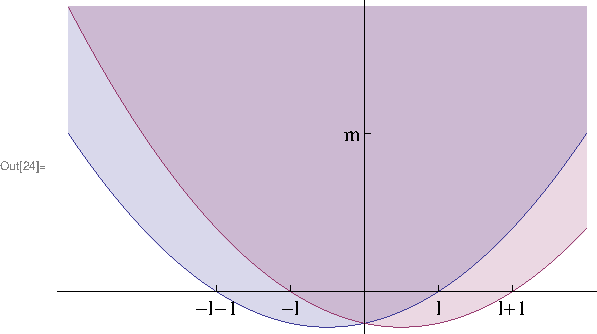
\includegraphics[scale=0.9]{solumom}    
  \end{center}

}

\frame{\frametitle{Conclusão}
$$L_-|l-l\rangle =C_-(l,-l)|l(-l-1)\rangle =\sqrt{(l-l)(2l+1)}|l(-l-1)\rangle=0$$

$$L_+|l-l\rangle =C_+(l,l)|l(l+1)\rangle =\sqrt{(l-l)(2l+1)}|l(-l-1)\rangle=0$$

Quais são os possíveis valores de $l$?

$m$ varia no mínimo em uma unidade, para ir de $-l$ até $l$ precisamos
de $2l$ passos. Se $2l$ é impar $l$ é semi-inteiro, se $2l$ é par 
$l$ é inteiro.
}

\frame{\frametitle{Representação em Posição}

É mais conveniente trabalhar em coordenadas esféricas. Para isto vamos escrever 
os operados relevantes nestas coordenadas. 

$$\frac{\partial}{\partial y}=\frac{\partial r}{\partial y}\frac{\partial}{\partial r}+ \frac{\partial \theta}{\partial y}\frac{\partial}{\partial \theta}+ \frac{\partial \phi}{\partial y}\frac{\partial}{\partial \phi}$$

$$r=\sqrt{x^2+y^2+z^2} \quad\theta=\tan^{-1} \frac{\sqrt{x^2+y^2}}{z}\quad \phi=\tan^{-1} \frac{y}{x} $$
}

\frame{\frametitle{Representação em Posição}

$$\frac{\partial r}{\partial x}=\frac{x}{r} \quad 
\frac{\partial \theta}{\partial x}=\frac{xz}{r^2\sqrt{x^2+y^2}}\quad
\frac{\partial \phi}{\partial x}=\frac{-y}{x^2+y^2}$$

$$\frac{\partial r}{\partial y}=\frac{y}{r} \quad 
\frac{\partial \theta}{\partial y}=\frac{yz}{r^2\sqrt{x^2+y^2}}\quad
\frac{\partial \phi}{\partial y}=\frac{x}{x^2+y^2}$$

}

\frame{\frametitle{Representação em Posição}
$$x\frac{\partial}{\partial y}-y\frac{\partial}{\partial x}=$$

$$=\left( \frac{yx-xy}{r}\right)\frac{\partial}{\partial r}+
\left( \frac{xyz-xyz}{r^2(x^2+y^2)}\right)\frac{\partial}{\partial \theta}+
\left( \frac{x^2+y^2}{x^2+y^2}\right)\frac{\partial}{\partial \phi}$$

$$=\frac{\partial}{\partial \phi}$$

$$L_z=\frac{\hbar}{i}\frac{\partial}{\partial \phi}$$
}


\frame{\frametitle{Representação em Posição}
$$L_\pm =\hbar e^{\pm i\phi}\left(\pm\frac{\partial}{\partial \theta}+i\frac{1}{\tan \theta} \frac{\partial}{\partial \phi} \right)$$


$$L^2=-\hbar^2\left(\frac{\partial^2}{\partial \phi^2}+\frac{1}{\tan \theta}
\frac{\partial}{\partial \theta} +\frac{1}{\sin ^2 \theta }\frac{\partial^2}{\partial \theta^2} \right)$$
}

\frame{\frametitle{Representação em Posição}
$$Y_{lm}(\theta, \phi)=\langle \theta\phi|lm\rangle $$

$$I=\int_0^{\pi}\int_0^{2\pi}d\theta d\phi \sin \theta |\theta\phi\rangle\langle \theta\phi|$$

$$\langle\theta^\prime\phi^\prime|\theta\phi\rangle=\frac{1}{\sin \theta}\delta(\theta-\theta^\prime)\delta(\phi-\phi^\prime)$$

}

\frame{\frametitle{Autofunções}
$$\langle \theta\phi | L_z| lm\rangle =\hbar m \langle \theta\phi|lm\rangle =\hbar m Y_{lm}(\theta,\phi )$$

$$L_zY_{lm}=\frac{\hbar}{i}\frac{\partial Y_{lm}}{\partial \phi}=\hbar m Y_{lm}(\theta, \phi)$$

$$Y_{lm}(\theta,\phi)=F(\theta)e^{im\phi}$$

}

\frame{\frametitle{Autofunções}
$$L_+ |ll\rangle =0$$

$$\langle\theta\phi | L_+ |ll\rangle =0$$

$$\hbar e^{i\phi}\left(\frac{\partial}{\partial \theta}+i\frac{1}{\tan \theta} \frac{\partial}{\partial \phi} \right)(e^{il\phi}F(\theta))=0$$

$$\frac{\partial F(\theta)}{\partial \theta}=\frac{l}{\tan \theta}F(\theta)$$

$$F(\theta ) =(\sin \theta)^l$$

}

\frame{\frametitle{Autofunções}
$$Y_{lm}(\theta,\phi )=CL_-^{l-m}(e^{il\phi}\sin \theta )^l$$
$$=Ce^{-i\phi}\left(-\frac{\partial}{\partial \theta}+i\frac{1}{\tan \theta} \frac{\partial}{\partial \phi} \right)^{l-m}[e^{il\phi}\sin^l \theta]$$
}

\frame{\frametitle{Normalização}

$C$ pode ser obtido normalizando a função.

$$\int_0^\pi\int_0^{2\pi} d\theta d\phi \sin \theta Y_{lm}(\theta,\phi )
Y^*_{lm}(\theta, \phi)=1$$
 
}

\frame{\frametitle{Esféricos Harmônicos}
$$
 Y_{00}=\frac{1}{2 \sqrt{\pi }}
$$

$$
 Y_{11}=\frac{1}{2} e^{i \phi } \sqrt{\frac{3}{2 \pi }} \sin (\theta ) \quad
 Y_{10}=-\frac{1}{2} \sqrt{\frac{3}{\pi }} \cos (\theta ) 
$$

$$
 Y_{1-1}=-\frac{1}{2} e^{-i \phi } \sqrt{\frac{3}{2 \pi }} \sin (\theta )
$$
}

\frame{\frametitle{Esféricos Harmônicos}
$$
 Y_{22}=\frac{1}{4} e^{2 i \phi } \sqrt{\frac{15}{2 \pi }} \sin ^2(\theta ) \quad
 Y_{21}=-\frac{1}{2} e^{i \phi } \sqrt{\frac{15}{2 \pi }} \cos (\theta ) \sin (\theta ) 
$$

$$
 Y_{20}=\frac{1}{16} \sqrt{\frac{5}{\pi }} (6 \cos (2 \theta )+2) \quad
 Y_{2-1}=\frac{1}{4} e^{-i \phi } \sqrt{\frac{15}{2 \pi }} \sin (2 \theta ) \quad
$$
$$
 Y_{2-2}=\frac{1}{4} e^{-2 i \phi } \sqrt{\frac{15}{2 \pi }} \sin ^2(\theta )
$$
}


\frame{\frametitle{$|Y_{lm}|^2$}
  \begin{center}
   \includegraphics[scale=0.2]{sphericalharmonics.png}
  \end{center}

}
\end{document}
